\documentclass{article}
\usepackage{graphicx,amsmath,latexsym}
\usepackage{color,psfrag,boxedminipage,amssymb}
%\usepackage[latin1]{inputenc}
%\usepackage[swedish]{babel}
%\usepackage{draftcopy}
\usepackage{tikz}
\usepackage{pgf}
\usetikzlibrary{positioning,arrows}

\newcommand{\st}{\ensuremath{\boldsymbol{s}_k(\boldsymbol{\theta})}}
\newcommand{\St}{{\mathbf S}\ensuremath{(\boldsymbol{\theta})}}
\newcommand{\phibf}{\ensuremath{\boldsymbol{\phi}}}
\newcommand{\varphibf}{\ensuremath{\boldsymbol{\varphi}}}
\def \phibfh{\ensuremath{\hat{\boldsymbol{\phi}}}}
\renewcommand{\sp}{\ensuremath{\boldsymbol{s}(\boldsymbol{\phi})}}
\newcommand{\hp}{\ensuremath{\boldsymbol{h}(\boldsymbol{\phi})}}
\newcommand{\thk}{\ensuremath{\boldsymbol{\theta}_k}}
\renewcommand{\th}{\ensuremath{\boldsymbol{\theta}}}
\newcommand{\alp}{\ensuremath{\boldsymbol{\alpha}}}
\def \thh{\ensuremath{\hat{\boldsymbol{\theta}}}}
\def \epsbf{\ensuremath{\boldsymbol{\epsilon}}}
\def \tht{\tilde{\th}}
\newcommand{\mubf}{\ensuremath{\boldsymbol{\mu}}}

\newcommand{\ctft}{\buildrel{{\cal F}}\over{\longleftrightarrow}}
\newcommand{\defin}{\buildrel{\triangle}\over{=}}

\def \Em{{\mathbb{E}}}



\def \abf{{\mathbf a}}
\def \Abf{{\mathbf A}}
\def \bbf{{\mathbf b}}
\def \Bbf{{\mathbf B}}
\def \cbf{{\mathbf C}}
\def \Cbf{{\mathbf C}}
\def \dbf{{\mathbf d}}
\def \Dbf{{\mathbf D}}
\def \ebf{{\mathbf e}}
\def \Ebf{{\mathbf E}}
\def \fbf{{\mathbf f}}
\def \Fbf{{\mathbf F}}
\def \gbf{{\mathbf g}}
\def \Gbf{{\mathbf G}}
\def \hbf{{\mathbf h}}
\def \Hbf{{\mathbf H}}
\def \ibf{{\mathbf i}}
\def \Ibf{{\mathbf I}}
\def \jbf{{\mathbf j}}
\def \Jbf{{\mathbf J}}
\def \kbf{{\mathbf k}}
\def \Kbf{{\mathbf K}}
\def \lbf{{\mathbf l}}
\def \Lbf{{\mathbf L}}
\def \mbf{{\mathbf m}}
\def \Mbf{{\mathbf M}}
\def \nbf{{\mathbf n}}
\def \Nbf{{\mathbf N}}
\def \obf{{\mathbf o}}
\def \Obf{{\mathbf O}}
\def \pbf{{\mathbf p}}
\def \Pbf{{\mathbf P}}
\def \qbf{{\mathbf q}}
\def \Qbf{{\mathbf Q}}
\def \rbf{{\mathbf r}}
\def \Rbf{{\mathbf R}}
\def \sbf{{\mathbf s}}
\def \Sbf{{\mathbf S}}
\def \tbf{{\mathbf t}}
\def \Tbf{{\mathbf T}}
\def \ubf{{\mathbf u}}
\def \Ubf{{\mathbf U}}
\def \vbf{{\mathbf v}}
\def \Vbf{{\mathbf V}}
\def \wbf{{\mathbf w}}
\def \Wbf{{\mathbf W}}
\def \xbf{{\mathbf x}}
\def \Xbf{{\mathbf X}}
\def \ybf{{\mathbf y}}
\def \Ybf{{\mathbf Y}}
\def \zbf{{\mathbf z}}
\def \Zbf{{\mathbf Z}}
\def \0bf{{\mathbf 0}}

\def \Emean{\mathbb{E}}

\def \Sibf{{\mathbf \Sigma}}
\def \xbbf{\mathbf{\bar{x}}}
\def \etr{\mbox{etr}}
\def \tr{\mbox{tr}}
\def \Tr{\mbox{Tr}}
\def \Cov{\mbox{Cov}}
\def \cost{\mbox{cost}}
\def \diag{\mbox{diag}}
\def \Lambf{{\mathbf{\Lambda}}}
\def \Gambf{{\mathbf{\Gamma}}}
\def \Sigbf{{\mathbf \Sigma}}
\newcommand{\rhobf}{\ensuremath{\boldsymbol{\rho}}}
\newcommand{\lambf}{\ensuremath{\boldsymbol{\lambda}}}
\newcommand{\nubf}{\ensuremath{\boldsymbol{\nu}}}

\newcounter{examplenr}[section]
\renewcommand{\theexamplenr}{\arabic{examplenr}}%{\thesection.\arabic{examplenr}}
\newenvironment{example}[1]{\vskip \baselineskip
\refstepcounter{examplenr}\noindent{{\bf
Example~\theexamplenr}\hskip .5em #1\\} }{\hrulefill $\Box$
 \vskip\baselineskip}



\newcounter{theoremnr}[section]
%\renewcommand{\thetheoremnr}{\thesection.\arabic{theoremnr}}
\renewcommand{\thetheoremnr}{\arabic{theoremnr}}
\newtheorem{A}[theoremnr]{Theorem}
\newcounter{theoremProofnr}[section]
%\renewcommand{\thetheoremProofnr}{\thesection.\arabic{theoremProofnr}}
\renewcommand{\thetheoremProofnr}{\arabic{theoremProofnr}}
\newtheorem{B}[theoremProofnr]{Proof of Theorem}
\newcounter{corollarynr}[section]
\renewcommand{\thecorollarynr}{\thesection.\arabic{corollarynr}}
\newtheorem{C}[corollarynr]{Corollary}
\newcounter{Lemmanr}[section]
\renewcommand{\theLemmanr}{\thesection.\arabic{Lemmanr}}
\newtheorem{D}[Lemmanr]{Lemma}
\newcounter{LemmaProofnr}[section]
\renewcommand{\theLemmaProofnr}{\thesection.\arabic{LemmaProofnr}}
\newtheorem{E}[LemmaProofnr]{Proof of Lemma}

\newcounter{propositionnr}[section]
\renewcommand{\thepropositionnr}{\arabic{propositionnr}}
\newtheorem{F}[propositionnr]{Proposition}
\newcounter{propositionProofnr}[section]
\renewcommand{\thepropositionProofnr}{\arabic{propositionProofnr}}
\newtheorem{G}[propositionProofnr]{Proof of proposition}

\newenvironment{working}{\color{blue}\sffamily\em}{}
\newenvironment{forslag}{\color{red}\sffamily\em}{}

\newcounter{definnr}[section]
\renewcommand{\thedefinnr}{\arabic{definnr}}
\newtheorem{J}[definnr]{Definition}



\usepackage{amsmath}
\usepackage{geometry}
\usepackage{caption}
\usepackage{lipsum}
\usepackage{hhline}
\geometry{a4paper}
\usepackage[backend=biber,style=ieee]{biblatex}
\bibliography{ref.bib}
\usepackage{comment}
\usepackage{multirow,array,units}

\usepackage{fancyhdr}

\pagestyle{fancy}
\fancyhf{}
\rhead{bvc981}
\lhead{Dhruv Chauhan}

\newenvironment{redmatrix}
  {\left(\array{@{}rrr|ccc@{}}}
  {\endarray\right)}
\newenvironment{ropmatrix}
  {\array{@{}c@{}}}
  {\endarray}
\newcommand\opone[2]{\xrightarrow{(#1)\times r_#2}}
\newcommand\optwo[3]{\xrightarrow{r_#1{}+{} #2r_#3}}

\begin{document}
\title{Machine Learning Assignment 5}
\author{Dhruv Chauhan}
\maketitle

\section{Neural Networks}
\subsection{Neural network implementation}

\newpage
\subsection{Neural network training}

The plots were attempted to be combined, but due to the number of lines they became difficult to understand, so I instead include the graphs on the next page, for 2 and 20 hidden neurons, and with learning rates of $[0.01, 0.1, 0.5, 1, 3]$. \\

Looking at the graphs, for small learning rates the error takes a long time to converge, (around 1000 epochs for 0.01). With a bigger learning rate the rate converges much faster, but at a local minimum that is higher than with lower rates (see learning rate of 3 for example).\\



\newpage
Below are the graphs for the input values [-10...10], (excluding 0 due to the division error in the sinc function) with the trained neural network and the sinc function, for both 2 and 20 hidden neurons.

\begin{figure}[h]
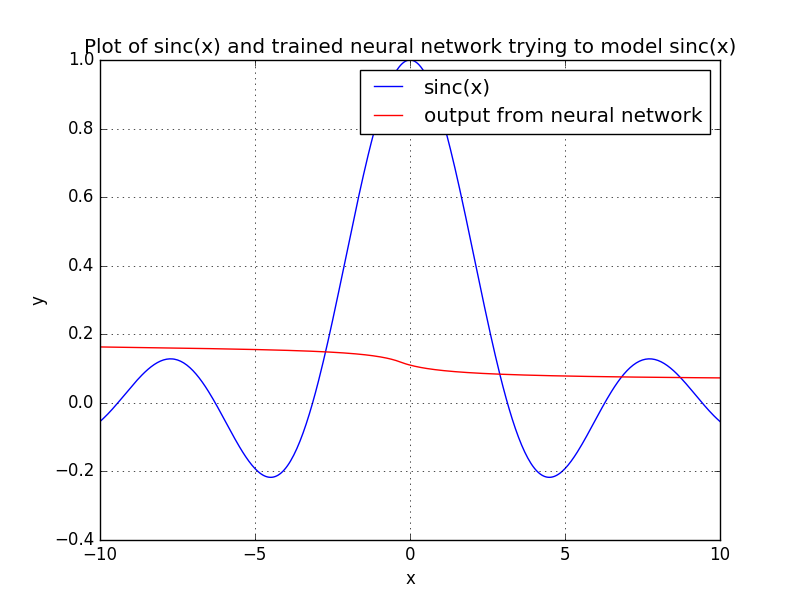
\includegraphics[width=16cm]{figs/nn2.png}
\caption{Neural Network trained with 2 Hidden Neurons}
\label{fig:nn2}
\end{figure}

\begin{figure}[h]
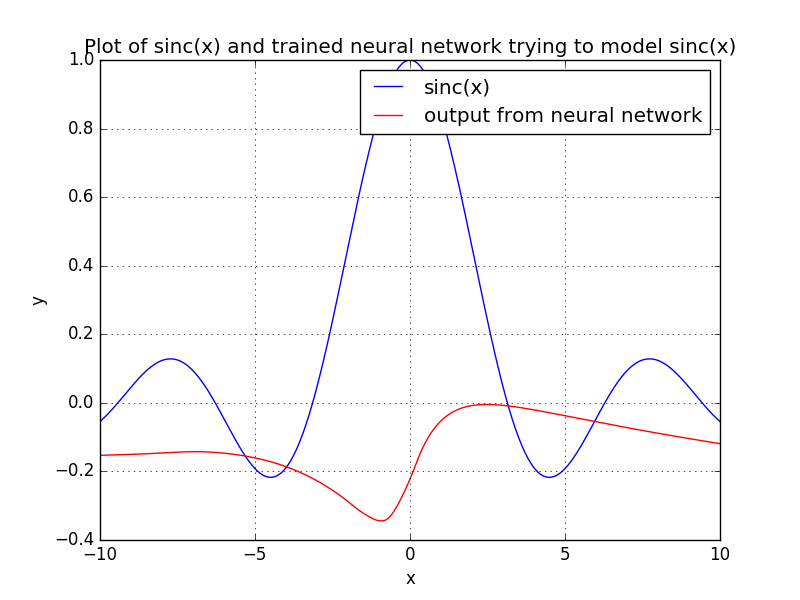
\includegraphics[width=16cm]{figs/nn20.png}
\caption{Neural Network trained with 20 Hidden Neurons}
\label{fig:nn20}
\end{figure}

Both models seemed to have missed the actual result by a bit, but the model with 2 hidden neurons roughly averages out the function, except around 0. The one with 20 hidden neurons oddly doesn't seem more accurate, although in total it crosses the true graph more times. Overfitting seemed to occur with a very low learning rate and a high number of epochs. We know that over fitting is occuring when the error rate on the validation set starts to increase again. By using early-stopping we prevent the over-training / this increase in error rate, and as a result we get a more suitable network for the function we are trying to model. We attempt to minimise the mean-squared error (until a noticeable convergence occurs), and before the error starts to increase again. 

\newpage
\section{The growth function}

\subsection{}

\subsection{}

\subsection{}

\subsection{}

\subsection{}

\newpage
\section{VC-Dimension}

\subsection{}

\subsection{}

\end{document}
